\documentclass[conference]{IEEEtran}
\IEEEoverridecommandlockouts

\usepackage{cite}
\usepackage{amsmath,amssymb,amsfonts}
\usepackage{algorithmic}
\usepackage{graphicx}
\usepackage{textcomp}
\usepackage{xcolor}
\usepackage[T1]{fontenc}
\usepackage{hyperref} % for hyperlinks

\def\BibTeX{{\rm B\kern-.05em{\sc i\kern-.025em b}\kern-.08em
    T\kern-.1667em\lower.7ex\hbox{E}\kern-.125emX}}

\begin{document}

\title{Automatic Motif Detection in the Star Wars Soundtrack\\
\vspace{0.2cm}
{\footnotesize 25 March 2025}}

\author{
\IEEEauthorblockN{Siddharth Saxena}
\IEEEauthorblockA{\textit{Universitat Pompeu Fabra}\\
Barcelona, Spain\\
siddharth.saxena01@estudiant.upf.edu}
\and
\IEEEauthorblockN{Andreas Papaeracleous}
\IEEEauthorblockA{\textit{Universitat Pompeu Fabra}\\
Barcelona, Spain\\
andreas.papaeracleous01@estudiant.upf.edu}
\and
\IEEEauthorblockN{Fernando Garcia de la Cruz}
\IEEEauthorblockA{\textit{Universitat Pompeu Fabra}\\
Barcelona, Spain\\
fernando.garcia11@estudiant.upf.edu}
}

\maketitle

\begin{abstract}
This project addresses the challenge of automatically detecting recurring musical motifs in film soundtracks by focusing on the Star Wars dataset. Our dual strategy begins with the extraction of melody information from audio recordings using two contrasting techniques: the CREPE deep-learning model and the signal processing-based Melodia algorithm. We then align these audio features with symbolic thematic data from XML files parsed via \texttt{music21}. For motif detection, we experiment with the stumpy matrix profile method—which offers fast candidate discovery—and Dynamic Time Warping (DTW), which, although computationally heavier, provides precise temporal alignments. Early findings indicate that while stumpy achieves acceptable accuracy with better speed, DTW’s detailed alignments come at a significant computational cost. We further explore motif comparisons across different audio tracks to identify recurrent patterns. Although challenges remain (such as data synchronization between noisy audio and cleaner symbolic data, and hyper-parameter tuning), our hybrid approach demonstrates promise for advancing musical pattern discovery in orchestral soundtracks.
More details about the code can be found in our GitHub repository\footnote{\url{https://github.com/SidSaxena01/Motif-Discovery}}.
\end{abstract}

\begin{IEEEkeywords}
Motif detection, matrix profile, dynamic time warping, CREPE, Melodia, symbolic music analysis.
\end{IEEEkeywords}

\section{Introduction}

\subsection{Background and Motivation}
Automatic motif detection is a central task in Music Information Retrieval (MIR), particularly for analyzing thematic material such as motifs and leitmotifs in film scores. These short, recurring patterns are not only crucial for musicological analysis but also for multimedia retrieval applications. However, variations in tempo, orchestration, and rhythm present significant challenges for automated detection. This project aims to bridge the gap between audio signal processing and symbolic music analysis by designing an end-to-end pipeline tailored to the Star Wars soundtrack.

\subsection{Project Objectives}
The key objectives of this project are to:
\begin{itemize}
    \item Develop an automated pipeline that integrates audio-based melody extraction and symbolic thematic alignment.
    \item Compare traditional motif detection methods (using matrix profiles via stumpy and DTW) on the Star Wars dataset.
    \item Evaluate motif detection accuracy by aligning known symbolic motifs with automatically extracted audio features.
    \item Investigate cross-track motif similarity to explore recurrent patterns across different audio recordings.
\end{itemize}

\subsection{Report Overview}
The report is organized as follows. Section II reviews related work and datasets in motif detection. Section III details our methodology for data extraction and motif detection. Section IV outlines the experimental setup and pipeline design. Section V presents preliminary results and analysis. Section VI discusses our findings, and Section VII offers directions for future research. Finally, Section VIII concludes the report.

\section{Related Work}

Previous studies have utilized both signal processing and deep learning approaches for motif detection. The matrix profile method has been successfully applied in exemplar works (e.g., Nuttall et al., 2023) for discovering repeated segments in time series data. Alternative methods—such as techniques replacing DTW with string matching (Ganguli et al., 2017)—demonstrate the value of symbolic abstraction in reducing computational complexity. More recent approaches have involved deep learning (Krause et al., 2021) to detect leitmotif activities. Our work builds on these foundations by applying these methods to film soundtracks and addressing data synchronization challenges.

The Star Wars thematic corpus\footnote{\href{https://github.com/Computational-Cognitive-Musicology-Lab/Star-Wars-Thematic-Corpus/}{Star Wars thematic corpus GitHub}} includes multiple themes available in symbolic formats (XML, Humdrum) along with time-stamped motif occurrences. In the broader MIR community, annotated datasets for orchestral music are limited, making motif annotation and detection an open challenge. This project not only validates motif detection techniques on a complex dataset but also contributes to improved annotation strategies.

\section{Methodology}

\subsection{Dataset Digitisation}
To enable subsequent processing of both audio and symbolic data, the initial dataset was converted into a digital format through the following steps:
\begin{itemize}
    \item \textbf{OCR Processing:} Raw text was extracted from \href{https://franklehman.com/starwars/}{Frank Lehman's Star Wars Thematic Catalogue PDF} using Optical Character Recognition.
    \item \textbf{Metadata Retrieval:} The YouTube API was employed to obtain track names associated with each YouTube link.
    \item \textbf{Data Mapping:} Fuzzy matching techniques, supplemented by a Large Language Model (LLM), were used to map motif names to their corresponding MusicXML files and to align YouTube titles with the available OST filenames on disk.
\end{itemize}
This digitisation process ensures that both symbolic and audio information are accurately aligned and ready for further analysis.

\subsection{Audio Stem Separation and Preprocessing}
Prior to melody extraction, audio tracks were decomposed into distinct stems using Demucs (model: \texttt{ht\_demucs\_ft}). This advanced deep-learning model separates the audio into vocals, bass, drums, and other components. Our experiments revealed that isolating the \textit{other} stem improved the results of melody extraction, as explicitly extracting the drums and bass allowed the models to focus on the most relevant melodic content. This preprocessing step benefits both the CREPE and Melodia models by enhancing the accuracy of pitch contour extraction.

\subsection{Data Sources and Preprocessing}
Our system leverages two complementary data sources:
\begin{itemize}
    \item \textbf{Symbolic Data:} MusicXML files are parsed using \texttt{music21} to extract thematic elements such as motifs and phrases. The resulting note sequences are transformed into time-aligned arrays, with interpolation strategies ensuring precise synchronization with audio-derived features.
    \item \textbf{Audio Data:} Raw audio files (WAV format) are processed to extract pitch contours. Preprocessing of audio includes normalization and resampling to 16~kHz, as required by the CREPE framework.
\end{itemize}

\subsection{Audio-Based Melody Extraction}
Two primary methods are employed for melody extraction:

\noindent\textbf{CREPE:}
\begin{itemize}
    \item Utilizes a deep-learning framework to estimate the primary pitch component from complex audio environments.
    \item Preprocessing involves normalizing the audio and resampling to 16~kHz.
\end{itemize}

\noindent\textbf{Melodia:}
\begin{itemize}
    \item Implements a signal processing approach that utilizes Viterbi encoding to extract the predominant melody.
    \item Despite its sensitivity to noise and overlapping sounds, Melodia is computationally efficient and yields clearer pitch contours, making it the preferred choice for our application.
\end{itemize}

\subsection{Motif Detection and Cross-Track Comparison}
\textbf{Motif Detection Techniques:}
\begin{itemize}
    \item \textbf{Stumpy (Matrix Profile):} The matrix profile is computed on the extracted pitch contours to rapidly identify candidate motifs. Hyper-parameters such as window length and exclusion zones were tuned experimentally.
    \item \textbf{Dynamic Time Warping (DTW):} To account for tempo variations and subtle interpretative differences in motif renditions, DTW is used for aligning time series data. While this method provides precise alignment, it incurs higher computational complexity and is applied primarily as a refinement tool.
\end{itemize}

\noindent\textbf{Cross-Track Motif Comparison:}
To explore motif recurrence across various audio tracks, pitch contour segments are compared using DTW (figure \ref{fig:dtw-match}) and pairwise similarity measures (e.g., via \texttt{stumpy.mass},  figure \ref{fig:mass}). This analysis (\ref{fig:dtw-warp}) aims to uncover recurrent motifs that appear consistently across multiple tracks, offering insights into thematic connections within the dataset.

\begin{figure}[htbp]
    \centering
    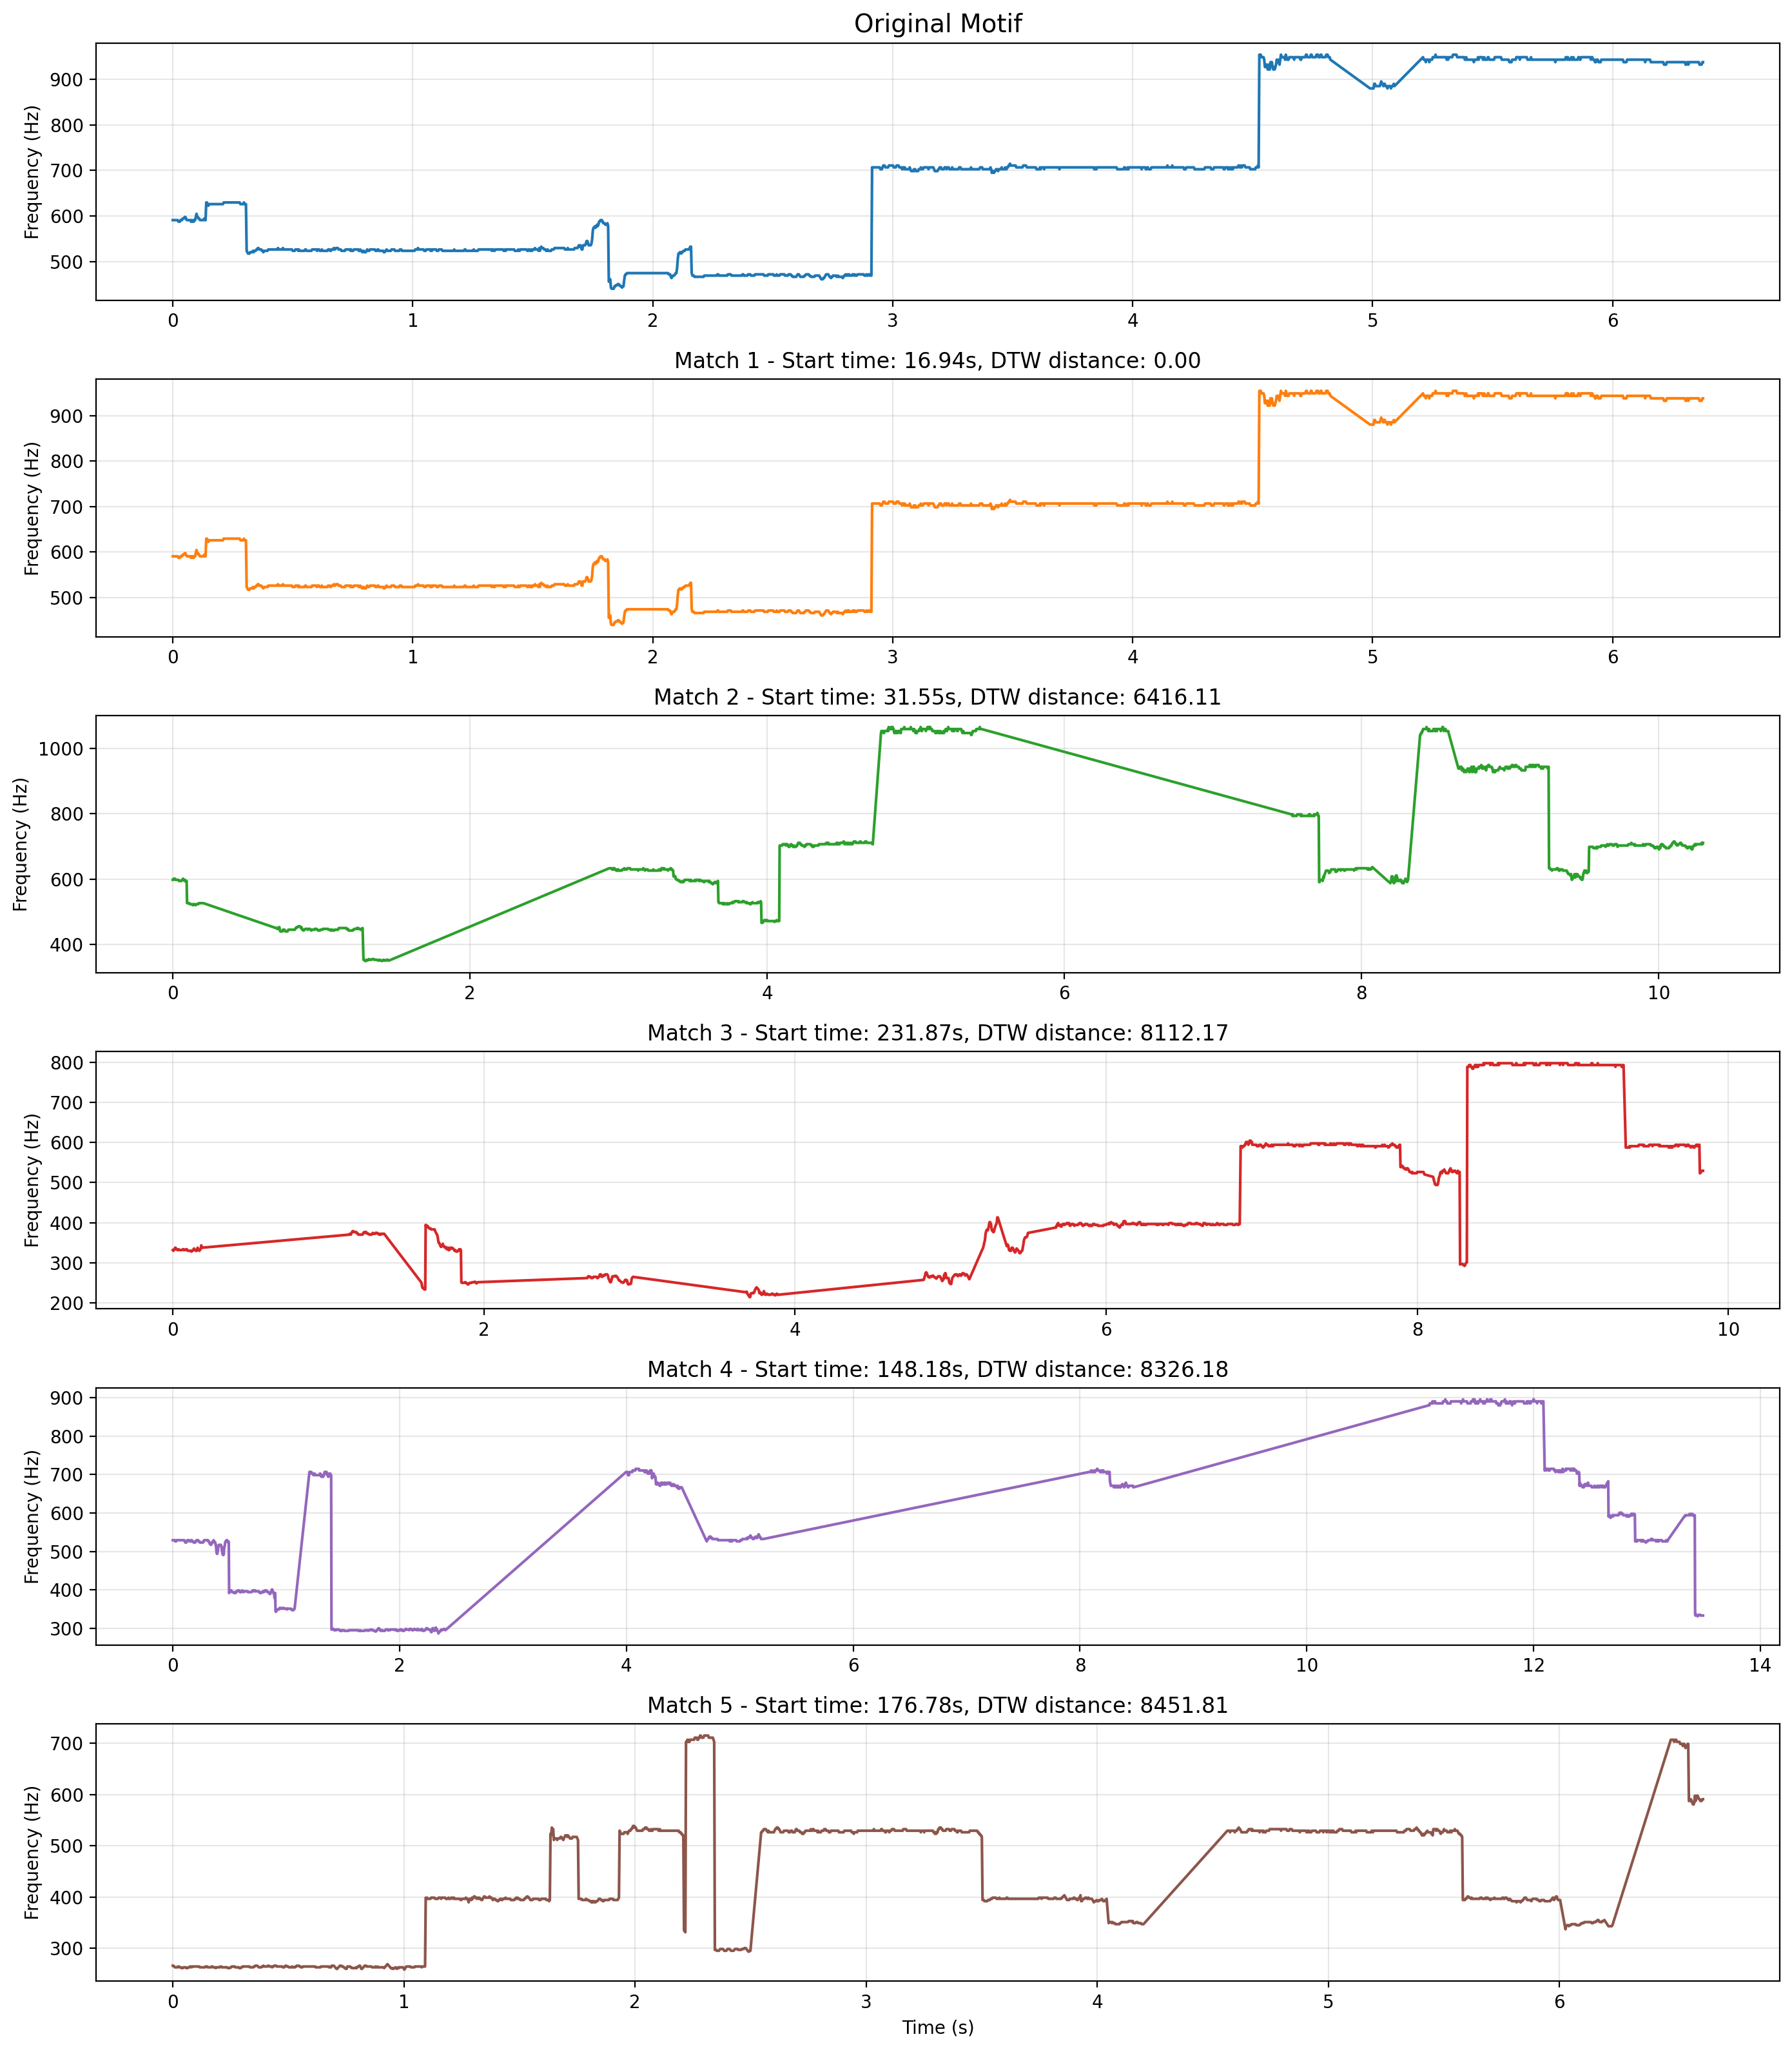
\includegraphics[width=0.9\linewidth]{figures/dtw-matches.png}
    \caption{DTW matches.}
    \label{fig:dtw-match}
\end{figure}

\begin{figure}[htbp]
    \centering
    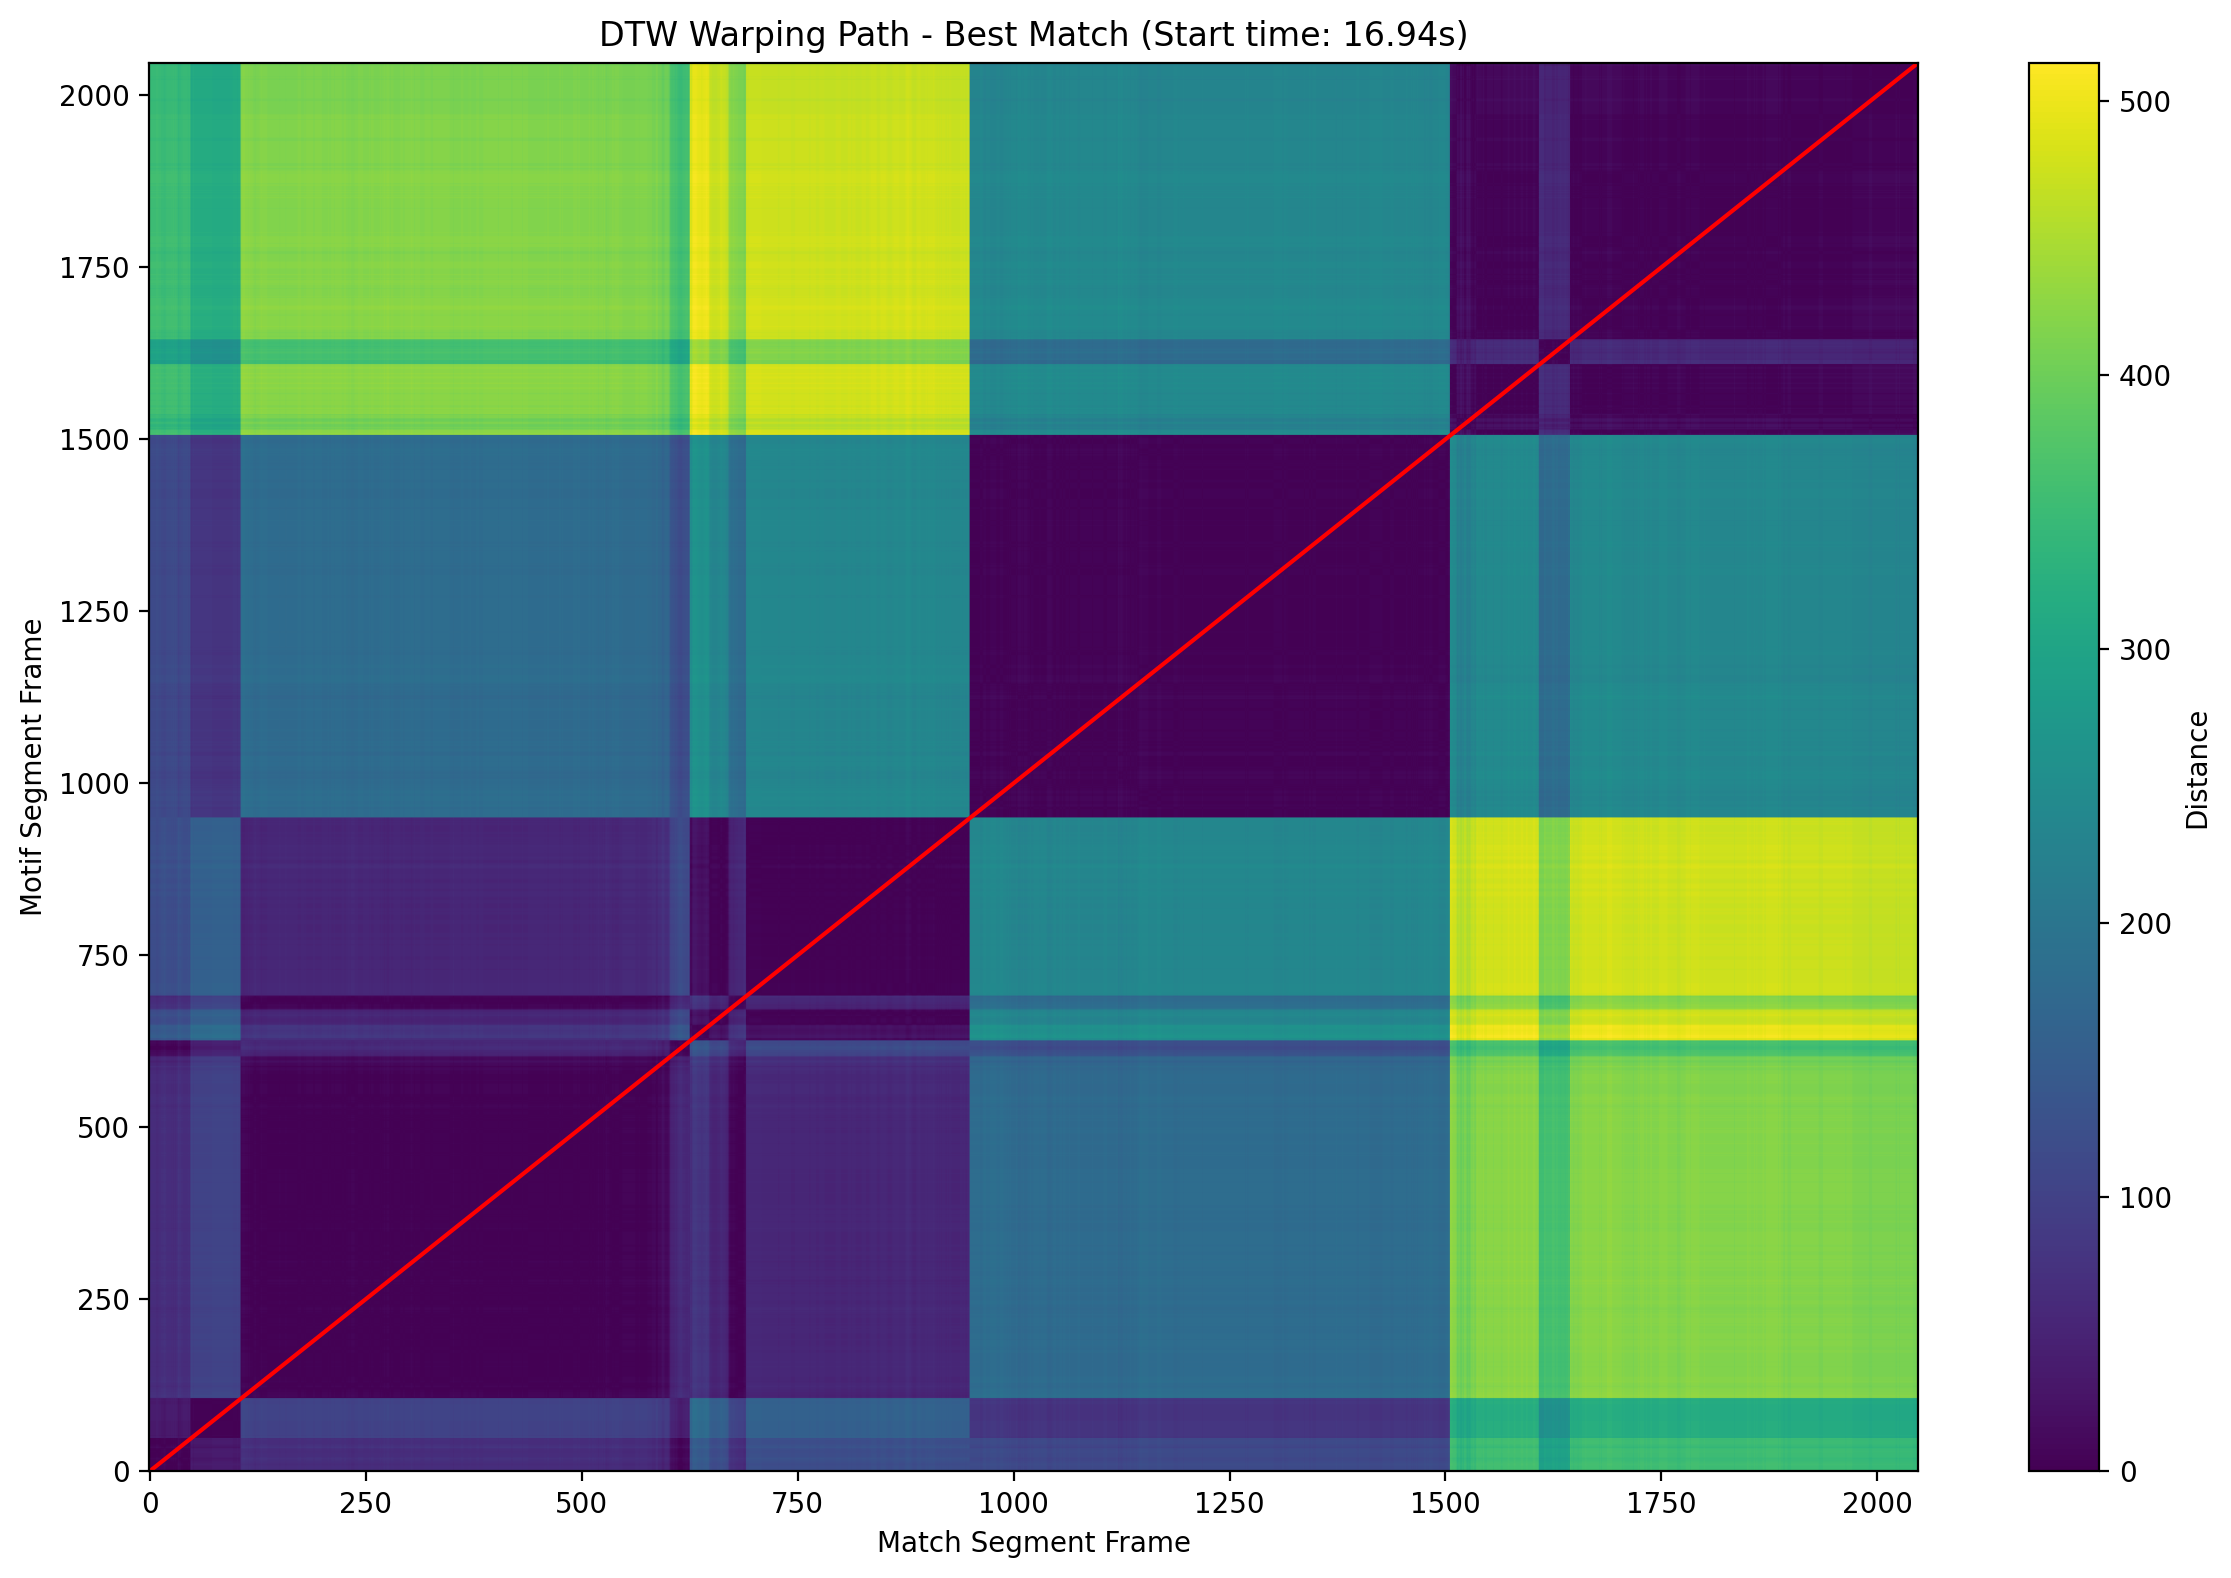
\includegraphics[width=0.9\linewidth]{figures/dtw-matches-warping-path.png}
    \caption{DTW warping path}
    \label{fig:dtw-warp}
\end{figure}

\begin{figure}[htbp]
    \centering
    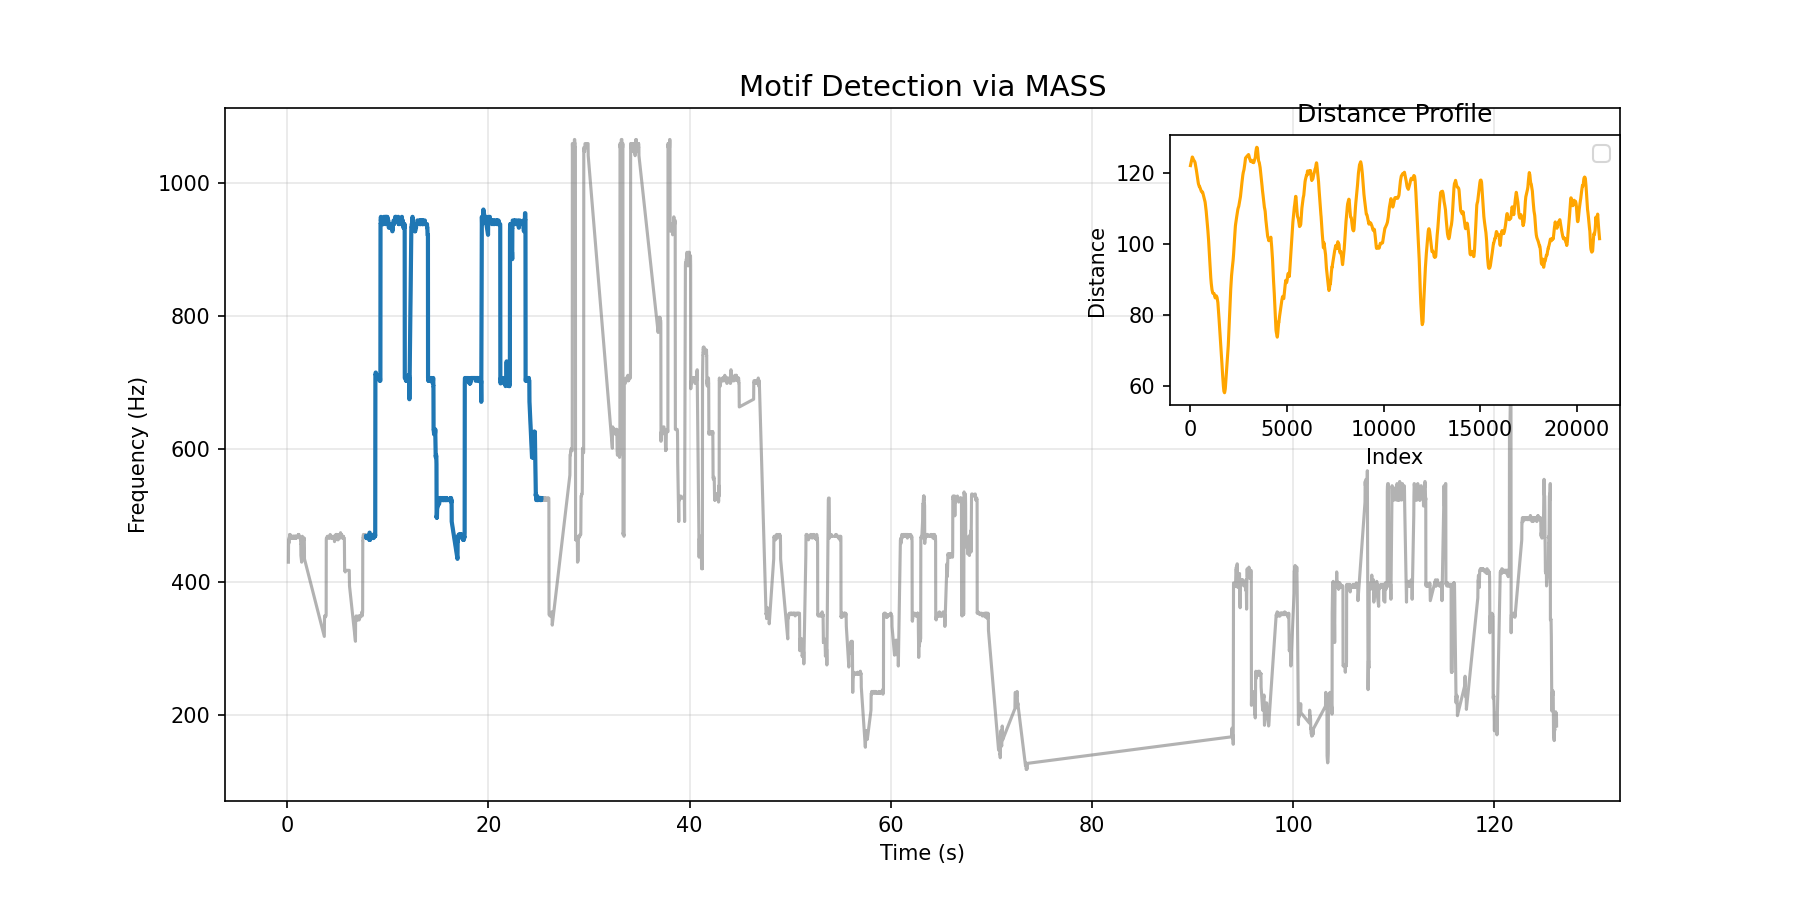
\includegraphics[width=0.9\linewidth]{figures/motif_detection_mass.png}
    \caption{Motif detection using mass algorithm.}
    \label{fig:mass}
\end{figure}

\section{Experimental Setup}

\subsection{Pipeline Design}
The end-to-end pipeline is designed as follows:
\begin{enumerate}
    \item \textbf{Input:} Star Wars audio recordings and corresponding XML files.
    \item \textbf{Stem Separation:} Each audio file is processed with Demucs (ht\_demucs\_ft) to separate the track into vocals, bass, drums, and other. For melody extraction, only the \textit{other} stem is used.
    \item \textbf{Thematic Extraction:} \texttt{music21} parses and transforms symbolic data into time-aligned arrays.
    \item \textbf{Melody Extraction:} Audio is processed via CREPE and Melodia to generate pitch contour arrays.
    \item \textbf{Data Transformation:} Align audio and symbolic data using BPM normalization and interpolation.
    \item \textbf{Motif Detection:} Apply the stumpy matrix profile method for candidate discovery and refine with DTW.
    \item \textbf{Cross-Track Comparison:} Identify recurrent motifs through pairwise alignment.
\end{enumerate}

A detailed flowchart of the pipeline is maintained in the project documentation.

\section{Experimental Results and Analysis}

\subsection{Performance of Melody Extraction}
Initial experiments reveal that CREPE is robust in polyphonic contexts due to its deep-learning basis, while Melodia provides clearer pitch contours in cleaner segments. Given the computational advantages, Melodia was chosen for further motif detection experiments.

\subsection{Motif Detection Results}
\begin{itemize}
    \item Known motifs were successfully detected in several tracks using the matrix profile method.
    \item Hyper-parameter sensitivity studies indicated that small changes significantly affect motif segmentation.
    \item DTW, while computationally intensive, improved temporal alignment of detected motifs.
\end{itemize}

\subsection{Cross-Track Motif Extraction}
Early experiments comparing motifs across different tracks have shown promising patterns of recurrence, although further validation and refinement are required.

\subsection{Challenges}
Major challenges include:
\begin{itemize}
    \item Synchronizing noisy audio-derived melody with more stable symbolic representations.
    \item Managing the high computational cost of DTW across large datasets.
    \item Tuning hyper-parameters in the matrix profile method to balance segmentation quality with efficiency.
\end{itemize}
Future work will focus on computational refinements and exploring adaptive parameter tuning strategies.

\section{Discussion}

\subsection{Interpretation of Preliminary Results}
The integration of audio-based extraction with symbolic thematic alignment validates our hybrid approach and provides a basis for further refinement. Some discrepancies remain between annotated motifs and automatically detected ones, highlighting the need for improved synchronization and parameter optimization.

\subsection{Comparison of Methods}
Stumpy offers rapid candidate motif detection and computational efficiency, though it is sensitive to parameter choices. In contrast, DTW yields more precise alignments at the expense of increased computational load. The trade-off between speed and accuracy is a key consideration in refining the pipeline.

\subsection{Limitations and Open Questions}
Current limitations include scalability challenges, dependency on manual hyper-parameter tuning, and difficulties in cross-track motif synchronization. Ongoing experiments aim to address these issues and clarify the ideal balance between various methods.

\section{Future Work}

\subsection{Pipeline Refinement}
Future work includes optimizing hyper-parameters via automated search methods and refining data synchronization techniques.

\subsection{Enhanced Cross-Track Analysis}
Planned experiments will focus on developing more robust methods for extracting and comparing recurrent motifs across audio tracks.

\subsection{Potential for Deep Learning Integration}
We plan to explore additional deep learning approaches to address limitations in DTW and matrix profile methodologies.

\subsection{Dataset Expansion and Annotation}
Additional manual annotations and dataset augmentation are intended to further ground and improve motif detection accuracy.

\section{Conclusion}
This report presents an end-to-end pipeline for automatic motif detection in the Star Wars soundtrack, integrating audio-based melody extraction with symbolic alignment. A key innovation of our approach is the incorporation of a Demucs-based stem separation step, which extracts the vocal, bass, and percussive elements out of the orchestral recordings to enhance melody extraction. Preliminary results demonstrate that combining this audio preprocessing with fast matrix profile methods and precise DTW alignment not only improves motif detection accuracy but also bolsters overall retrieval in complex orchestral recordings. Although challenges remain—especially in data synchronization, hyper-parameter tuning, and computational cost—the encouraging early findings suggest that our hybrid approach holds promise for advancing musical retrieval and analysis in film soundtracks. Future work will focus on refining these methods and validating improvements across larger datasets.

% References
\begin{thebibliography}{00}
\bibitem{Nuttall2023} T. Nuttall, G. Plaja-Roglans, L. Pearson, and X. Serra, ``The Matrix Profile for Motif Discovery in Audio—An Example Application in Carnatic Music,'' in \textit{Music in the AI Era}, M. Aramaki \textit{et al.}, Eds., vol. 13770, pp. 228--237, Springer, 2023, doi:10.1007/978-3-031-35382-6\_18.
\bibitem{Ganguli2017} K. K. Ganguli, A. Lele, S. Pinjani, P. Rao, A. Srinivasamurthy, and S. Gulati, ``Melodic shape stylization for robust and efficient motif detection in Hindustani vocal music,'' in \textit{Proc. 2017 Twenty-Third National Conference on Communications (NCC)}, pp. 1--6, 2017, doi:10.1109/NCC.2017.8077055.
\bibitem{Hao2013} Y. Hao, M. Shokoohi-Yekta, G. Papageorgiou, and E. Keogh, ``Parameter-Free Audio Motif Discovery in Large Data Archives,'' in \textit{Proc. 2013 IEEE 13th International Conference on Data Mining}, pp. 261--270, 2013, doi:10.1109/ICDM.2013.30.
\bibitem{Krause2021} M. Krause, M. Müller, and C. Weiß, ``Towards Leitmotif Activity Detection in Opera Recordings,'' \textit{Trans. Int. Soc. Music Inf. Retrieval}, vol. 4, no. 1, pp. 127--140, 2021, doi:10.5334/tismir.116.
\bibitem{DeFossez2019} A. Defossez, N. Usunier, L. Bottou, and F. R. Bach, ``Demucs: Deep Extractor for Music Sources with extra unlabeled data remixed,'' \textit{CoRR}, vol. abs/1909.01174, 2019.
\bibitem{Arthur2023} C. Arthur, F. Lehman, and J. McNamara, ``Presenting the SWTC: A Symbolic Corpus of Themes from John Williams' Star Wars Episodes I-IX,'' arXiv preprint arXiv:2309.03298, 2023. Available: \url{https://arxiv.org/abs/2309.03298}.
\end{thebibliography}

\section*{Appendix: Visualizations of Motif Detection Results}

\begin{figure}[htbp]
    \centering
    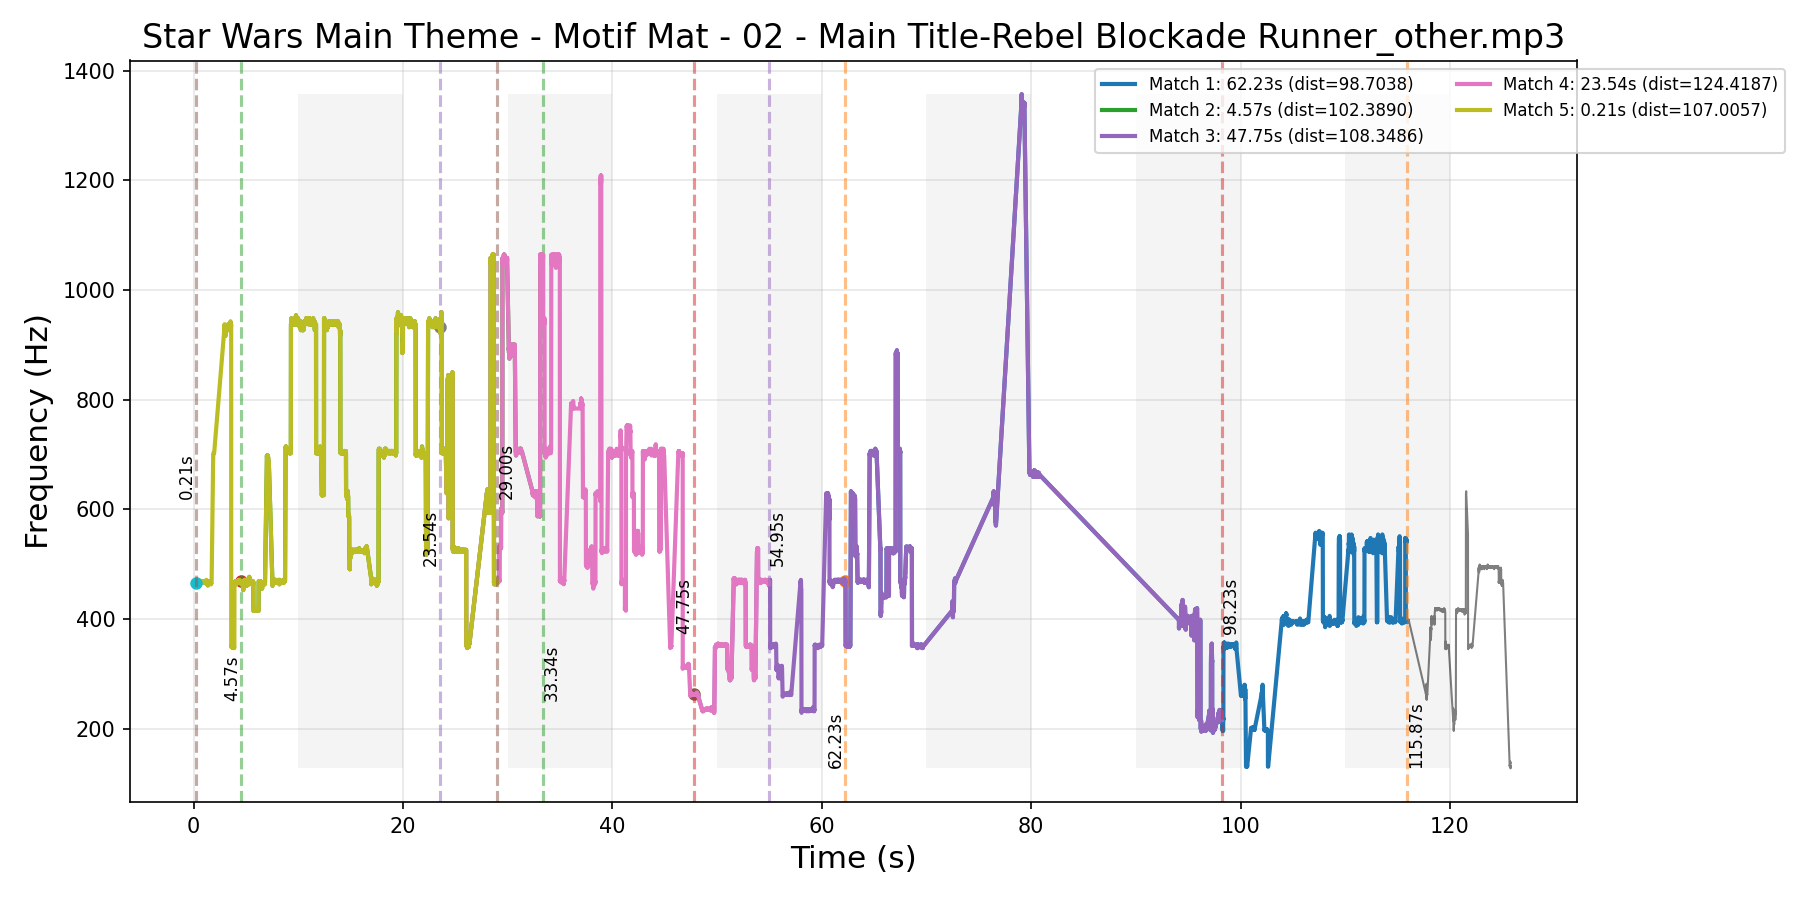
\includegraphics[width=0.9\linewidth]{figures/1a. MAIN THEME_Star Wars Episode IV A New Hope (1977) Soundtrack 02 Main Title _ Rebel Blockade _Runner Medley_motif_matches.png}
    \caption{Main motif detection in main theme.}
    \label{fig:themes}
\end{figure}

\enddocument
